\documentclass[12pt]{article}

\usepackage{amssymb}
\usepackage{caption}
\usepackage{subcaption}
\usepackage{float}
\usepackage{makecell}
\usepackage{amsmath}
\usepackage{graphicx}
\graphicspath{ {./images/} }
\usepackage[utf8]{inputenc}
\usepackage[russian]{babel}
\usepackage{geometry}
 \geometry{
 a4paper,
 left=20mm,
 right=20mm,
 top=20mm,
 bot=20mm,
 }

\begin{document}

\begin{titlepage}
\begin{center}
    {\small НАЦИОНАЛЬНЫЙ ИССЛЕДОВАТЕЛЬСКИЙ УНИВЕРСИТЕТ ИТМО} \\
    {\small Факультет систем управления и робототехники} \\
    \vspace*{10\baselineskip}
    {\LARGEМоделирование динамических систем} \\
    \ \\
    {\LARGEЛабораторная работа №6} \\
    \ \\
    {\LARGE Дескрипторный метод} \\
    \ \\
    Вариант 2 \\
    \vspace*{10\baselineskip}
    \hfill {\small Выполнил студент:} \\
    \hfill {\small Кирбаба Д.Д. R3338} \\
    \ \\
    \hfill {\small Преподаватель:} \\
    \hfill {\small Семенов Д.М.} \\
    \mbox{}
    \vfill {\smallг. Санкт-Петербург\\2023}
\end{center}
\end{titlepage}

\section*{Ход работы}
Дана система с произвольной постоянной задержкой $h$:
\[
    \dot{x}(t) = Ax(t) + A_1x(t - h),
\]
где $x \in \mathbb{R}, \ A = \begin{bmatrix}
    2 & -2 \\ 1 & 3
\end{bmatrix}, \ A_1 = \begin{bmatrix}
    -4 & 0 \\ -1 & -5
\end{bmatrix}.$

Промоделируем данную систему в при разных задержках. Выберем одно значение, при которой система будет устойчивой, и другое, при которой она будет неустойчивой.
\begin{figure}[H]
    \centering
    \subfloat[\centering устойчивый случай ($h=0.2$)]{{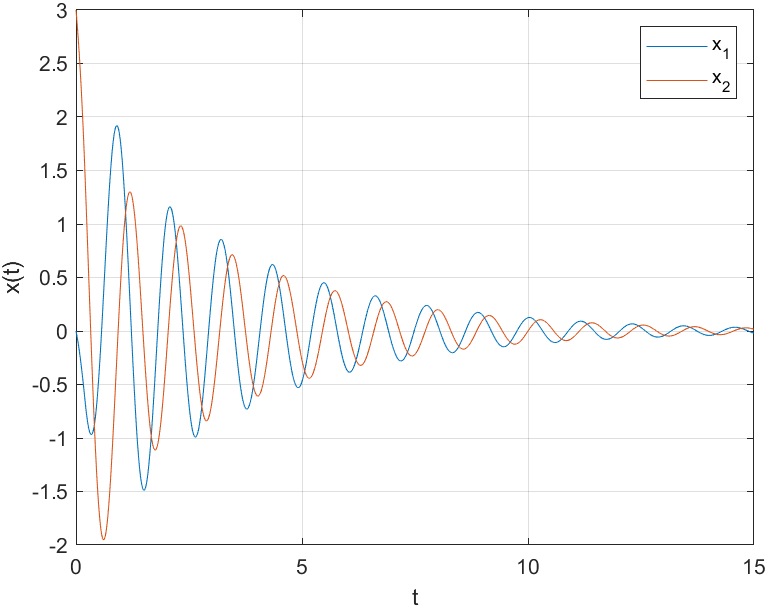
\includegraphics[width=0.45\textwidth]{stable.png} }}%
    \qquad
    \subfloat[\centering неустойчивый случай ($h=0.5)$]{{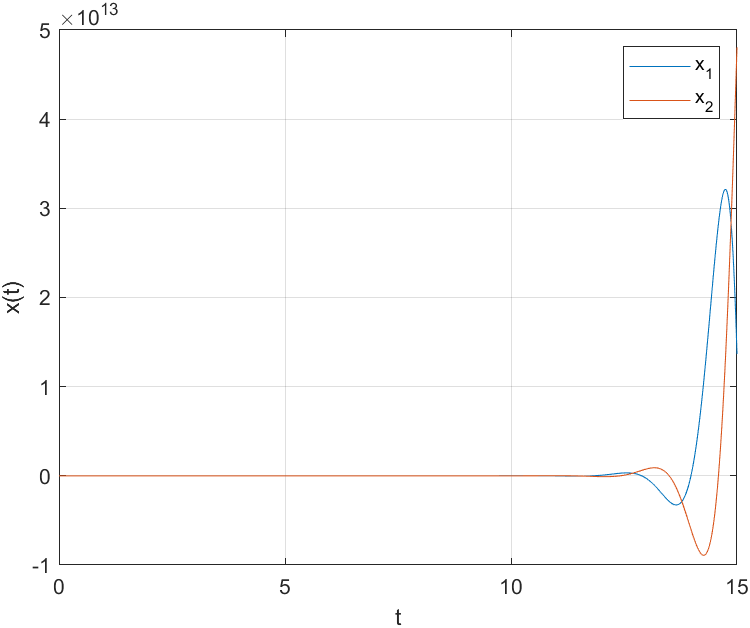
\includegraphics[width=0.45\textwidth]{unstable.png} }}%
    \caption{Моделирование системы при различных задержках.}%
    \label{fig:st_ust}
\end{figure}

Теперь, используя дескрипторный метод, найдем максимальную задержку, при которой данная система будет устойчивой. \\
Для этого необходимо решить следующую систему линейных матричных неравенств:
\[
    \begin{split}
        & \begin{bmatrix}
            \Psi & P-P_2^T(A+A_1)^TP_3 & -hP_2^TA_1 \\
            * & -P_3-P_3^T+hR & -hP_3^TA_1 \\
            * & * & -hR
        \end{bmatrix} < 0, \\
        & \Psi = P_2^T(A+A_1)+(A+A_1)^TP_2, \ P>0, \ R>0.
    \end{split}
\]
Здесь $P_2$ и $P_3$ – произвольные матрицы. В результате решения матричного неравенства в MATLAB получена максимальная задержка $h=0.211$, при которой система является устойчивой. \\
\ \\
Теперь построим регулятор $u(t) = Kx(t)$ такой, что замкнутая система
\[
    \dot{x}(t) = Ax(t) + A_1x(t-h) +Iu(t) = (A+K)x(t) + A_1 x(t-h)
\]
была устойчивой при любых задержках $h$. \\
Для этого достаточно решить матричное неравенство:
\[
    \begin{bmatrix}
        \Tilde{A}^TP + P\Tilde{A} + Q & PA_1 \\
        A_1^TP & -Q
    \end{bmatrix} < 0,
\]
где $P = P^T>0, \ Q=Q^T>0, \ \Tilde{A} = A+K$. \\
С помощью вычислений, нашли следующую матрицу:
\[
    K = 10^8* \cdot \begin{bmatrix}
        -7.3845 & 3.7655 \\
        3.7655 & -5.3991
        \end{bmatrix}
\]

\section*{Выводы}
В данной лабораторной работе был исследован дескрипторный метод для анализа систем с задержками. Суть данного метода в том, что он гарантирует устойчивость системы с запаздыванием при задержке, принадлежащей некоторому промежутку.\\
\ \\
В первой части работы, используя дескрипторный метод, было найдено максимальное значение задержки, при котором система остается устойчивой $h = 0.221 \ sec$. \\
Во второй части работы был синтезирован регулятор, стабилизирующий систему с любыми задержками. Для этого требовалось решить систему матричных неравенств, и для проверки устойчивости замкнутой системы использовать метод функционалов Ляпунова-Красовского. \\
\ \\
В результате, система с данным регулятором действительно устойчива.

\end{document}